\documentclass[paper=a4, fontsize=11pt, abstract=on]{scrartcl} % A4 paper and 11pt font size
\usepackage[left=2.5cm,top=2.5cm,right=2.5cm,bottom=2.5cm]{geometry} 
\usepackage{amsmath}
\usepackage[toc,page]{appendix}
\usepackage{graphicx}
\usepackage{sectsty}
\usepackage{amsfonts}
\usepackage{fancyhdr}
\pagestyle{fancyplain}
\usepackage{parskip}
\usepackage{subcaption}
\usepackage{wrapfig}
\usepackage[english]{babel}
\usepackage{bibentry}
\usepackage {natbib}
\usepackage{float}
\usepackage{hyperref}
\usepackage{listings}
  \usepackage{courier}
\usepackage{graphics}
 \usepackage{color} 
 \lstset{
         basicstyle=\footnotesize\ttfamily, % Standardschrift
         %numbers=left,               % Ort der Zeilennummern
         numberstyle=\tiny,          % Stil der Zeilennummern
         %stepnumber=2,               % Abstand zwischen den Zeilennummern
         numbersep=5pt,              % Abstand der Nummern zum Text
         tabsize=2,                  % Groesse von Tabs
         extendedchars=true,         %
         breaklines=true,            % Zeilen werden Umgebrochen
         keywordstyle=\color{red},
    		frame=b,         
 %        keywordstyle=[1]\textbf,    % Stil der Keywords
 %        keywordstyle=[2]\textbf,    %
 %        keywordstyle=[3]\textbf,    %
 %        keywordstyle=[4]\textbf,   \sqrt{\sqrt{}} %
         stringstyle=\color{white}\ttfamily, % Farbe der String
         showspaces=false,           % Leerzeichen anzeigen ?
         showtabs=false,             % Tabs anzeigen ?
         xleftmargin=17pt,
         framexleftmargin=17pt,
         framexrightmargin=5pt,
         framexbottommargin=4pt,
         %backgroundcolor=\color{lightgray},
         showstringspaces=false      % Leerzeichen in Strings anzeigen ?        
 }
 \lstloadlanguages{% Check Dokumentation for further languages ...
         %[Visual]Basic
         %Pascal
         C
         %Python
         %C++
         %XML
         %HTML
         %Java
 }
% \usepackage{caption}
% \DeclareCaptionFont{white}{\color{white}}
% \DeclareCaptionFormat{listing}{\colorbox[cmyk]{0.43, 0.35, 0.35,0.01}{\parbox{\textwidth}{\hspace{15pt}#1#2#3}}}
% \captionsetup[lstlisting]{format=listing,labelfont=white,textfont=white, singlelinecheck=false, margin=0pt, font={bf,footnotesize}}



\numberwithin{equation}{section}
\numberwithin{figure}{section} 
\numberwithin{table}{section}
%\setlength\parindent{0pt}

\fancyhead[R]{\thepage} 
\fancyhead[L]{Reyes, Adam} 
\fancyhead[C]{The Feigenbaum Number} 
\fancyfoot[L]{} 
\fancyfoot[C]{} 
\fancyfoot[R]{} 

\newcommand{\horrule}[1]{\rule{\linewidth}{#1}}

\title{	
The Feigenbaum Number
\horrule{0.5pt}
\normalfont \normalsize 
\textsc{Dynamics Fall 2013}
}

\author{Adam Reyes} % Your name

\date{\normalsize\today} % Today's date or a custom date


\begin{document}
\maketitle

\section{Introduction}
\label{sec:intro}

\begin{wrapfigure}{r}{.5\textwidth}
  \centering
  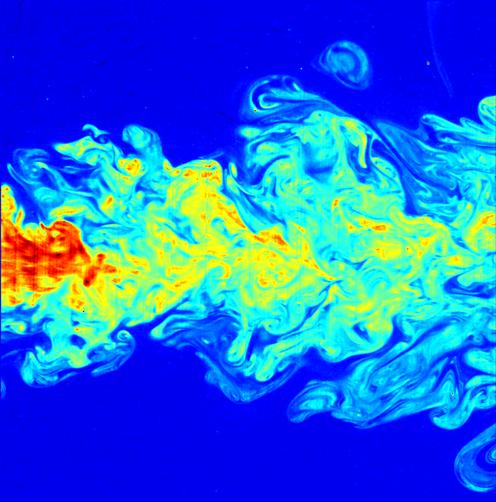
\includegraphics[width=.4\textwidth]{Jet}
  \caption{Example of turbulent fluid flow\cite{wiki}}
  \label{fig:turb}
\end{wrapfigure}

Physicist Werner Heisenberg said, should he meet 
God, he would ask: "Why relativity? And why turbulence? I really believe he will have
an answer for the first". Turbulence is a fluid phenomena that is
characterized by flow that changes chaotically (see
Figure~\ref{fig:turb}). Turbulent flow can be seen as a transition
from a smooth laminar flow to large vortices and finally to chaotic flow, as exhibited in
Figure~\ref{fig:turb}. In the turbulent regime you can find many small
scale vortices resembling those found in the less chaotic
regimes. This is reminiscent of phase transitions in states of matter,
where near a phase transition fluctuations appear the same in all
length scales, the idea of which was developed by Kenneth Wilson \cite{Wilson}.

\vline

The apparent order in the presence of smaller and smaller vortices in
turbulent flow lead Mitchell Feigenbaum, in the 1970s, to try and
apply the ideas of Wilson to the analysis of turbulent systems, and
more generally non-linear systems of equations. Feigenbaum began by
investigating the simplest of non-linear equations, the logistic map:

\begin{equation}
  \label{eq:logmap}
  x_{n+1} = r\cdot x_n \cdot (1 - x_n)
\end{equation}



\section{Maps}
\label{sec:map}

We will consider discrete maps (like the logistic map
Eq.\ref{eq:logmap}) that take some seed value, $x_0\in \mathbb{R}$, and sends it to
some value $x_n$ by the iterative action of some function $F$ $n$
times on the seed value:

\begin{equation}
  \label{eq:map}
  x_0 \rightarrow F^{(n)}(x_0) = x_n 
\end{equation}
Here $F^{(n)}$ refers to the composition of $F$ with itself,
$F \circ F(x_0)$, $n$ times. We might be interested in the fixed
points, $X\in \mathbb{R}$, of the map, such that:

\begin{equation}
  \label{eq:fixed}
  X = F(X)
\end{equation}
We can determine the stability of a fixed point by examining how the
map behaves in the region around $X$. For small $\epsilon_n$ such that
$x_n = X + \epsilon_n$, we can expand $F(x_n)$ around $F(X)$ in a
Taylor Series: 
\begin{equation}
  \label{eq:taylor}
  F(x_n) = F(X) + \epsilon_n F'(X) + \frac{1}{2}\epsilon_n^2F''(X) + \mathcal{O}(\epsilon_n^3)
\end{equation}
where $\mathcal{O}(\epsilon_n^3)$ refers to terms of order
$\epsilon_n^3$ or greater. We see that $X$ is stable, meaning nearby
seeds get mapped to $X$ as $\epsilon_n\rightarrow 0$, for $|F'(X)| <
1$. In this case the point $X$ is called an attractor. There are two
cases for which this condition of attraction is satisfied
\begin{enumerate}
\item $0 < |F'(X)| < 1$ \\
  In this case $F(x_n)$ converges with $\epsilon_n$, giving
  \emph{first-order convergence}.
\item $ F'(X) = 0$ and $F''(X)\not= 0$\\
  In this case $F(x_n)$ converges with $\epsilon_n^2$, giving
  \emph{second-order convergence}.
\end{enumerate}

\subsection{The Linear Map}
\label{sec:linmap}



The simplest map that can be imagined is the linear map, of the form
\begin{equation}
  \label{eq:linmap}
  x_{n+1} = rx_n
\end{equation}

It is easy to see that the behavior of the linear map is dependent on
the value of $r$. We have 
\begin{equation}
  \label{eq:linmap1}
  x_{n} = r^nx_0 = e^{n\ln x_0r} = x_0 e^{n\ln r}
\end{equation}
\begin{itemize}
\item $0\leq r < 1$\\
  $x_n\rightarrow 0$ $\forall x_0$\\
  0 is an attractor in this region of $r$, with all seed values sent to
  0.
\item $r=1$\\
  $x_n = x_0$ $\forall x_0$\\
  And there are now stable fixed points, as each seed value is mapped
  to a different point.
\item $r>1$\\
  $x_n\rightarrow \infty$ $\forall x_0$\\
  So $\infty$ is an attractor.
\end{itemize}

\subsection{The Logistic Map}
\label{sec:logmap}

Following from the linear map(Eq.\ref{eq:linmap}), the simplest
nonlinear map one might think of would take the form
\begin{equation}
  \label{eq:logmap2}
  x_{n+1} = ax_n - bx_n^2
\end{equation}
Using a simple change of variable, $x_n\rightarrow bx_n/r$, we can put
Eq.\ref{eq:logmap2} into the form of the logistic map
(Eq.\ref{eq:logmap}), with a single parameter, $r$.
We will restrict our discussion of the linear map to the values of $r$
that will map $x\in [0,1] \rightarrow [0,1]$. This restricts $r$ to
the interval $[0,4]$.

\vline

We can find the fixed points, $X$, of the logistic
map(Eq.\ref{eq:logmap}), by finding solutions to
Eq.\ref{eq:fixed}. Doing so we get $X=0$ and $X=1-1/r$. We get that
the derivative $F'(X) = r(1-2X)$. Plugging in our fixed points we get
\begin{align}
\begin{split}
  \label{eq:fixedderivs}
  F'(0) = & r \\
  F'(1-1/r) = & 2-r
\end{split}
\end{align}

We can now analyze the fixed points by using the derivative of
$F$(Eq.\ref{eq:fixedderivs}).
\begin{itemize}
\item We see that $X=0$ is a stable fixed point for $r\in [0,1)$, while
$X=1-1/r$ is not. 
\item But for $r\in (1,3)$, $X=0$ is now unstable, and $X=1-1/r$ is
  stable.
\item When $r\in (3,4]$ we have a situation very different from what
  we saw in the case of the linear map. In the previous two cases for
  $r$ we had one point being the stable and the other unstable,
  pushing $x_n$ towards the stable fixed point as $n\rightarrow
  \infty$. In this case both fixed points are unstable.
\end{itemize}

\section{Period-Doubling}
\label{sec:pdub}

In Section~\ref{sec:logmap} we showed that the fixed points of the
logistic map are both unstable in the region $r \in (3, 4]$. As $r$ is
increased stability with $n \rightarrow \infty$, will be exchanged
between the fixed points. 

\vline

We can also examine the points that satisfy
\begin{equation}
  \label{eq:doubling}
  x_{n+2} = F(x_{n+1})
\end{equation}
which leads to a polynomial of degree four, leaving four roots. Two of
which are of course our previous roots. This can be extended further
giving higher order polynomials and likewise more fixed points. As $r$
is increased the number of possible stable points will double on
certain intervals, the so-called \emph{period-doubling
  bifurcations}. So we have that as $r$ increases from 3 the stability
cascades through these bifurcations, until there are so many that the
mapping becomes extremely sensitive to small fluctuations between seed
values. This sensitivity to initial conditions is what leads this
region to be called chaotic. We can construct a \emph{bifurcation digram} by mapping a set
of seed values using the logistic map and plotting them over a range
of $r$'s. Such a diagram for the logistic map is given in
Figure~\ref{fig:logmap}. You can see how the stability is exchanged
between fixed points after $r=3$ and then is successively bifurcated
over $r$. 

\pagebreak

\begin{figure}[h]
  \centering
  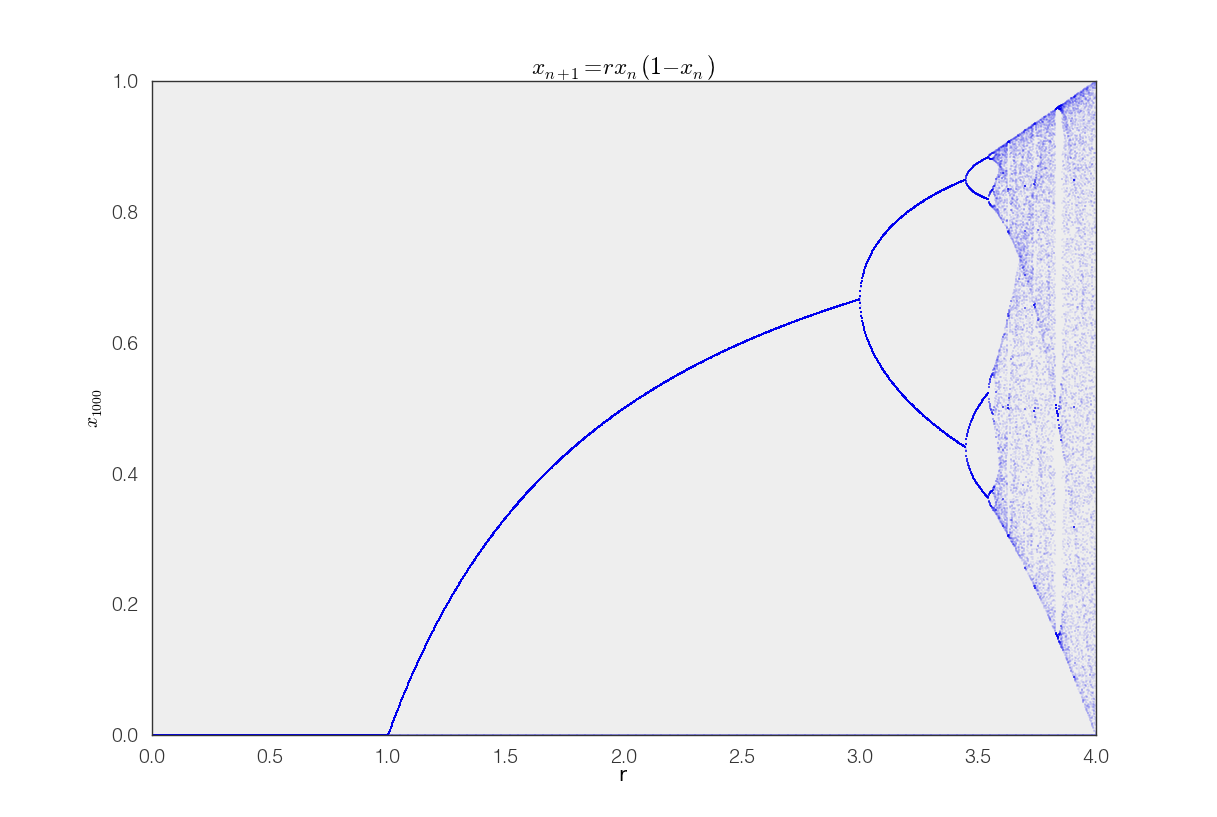
\includegraphics[width=0.85\textwidth]{logmap}
  \caption{Bifurcation diagram for the logistic map: $[0,1] \rightarrow [0,1]$, for $r \in (0, 4)$ }
  \label{fig:logmap}
\end{figure}


\section{The Feigenbaum Number $\delta=4.6692...$}
\label{sec:feig}

Feigenbaum was studying these bifurcations of the logistic map. He
discovered that the ratio of successive intervals between these
bifurcations approached some value asymptotically. That is
\begin{equation}
  \label{eq:feigen}
  \frac{a_n - a_{n-1}}{a_{n+1}-a_n} \rightarrow \delta
\end{equation}
$\delta$ is the Feigenbaum number, named for its discoverer. It is
given as 
$$
\delta = 4.6692016...\cite{kibble}
$$
As one might expect, Feigenbaum set out to see if other nonlinear maps
also had the ratio of their period-doubling bifurcation intervals
approach some value asymptotically. Not only did Feigenbaum discover
that this phenomena is exhibited in other nonlinear maps, but that
they all approached the same $\delta$\cite{feigenbaum}! An example of
another nonlinear map, the trigonometric map, is given in
Figure~\ref{fig:trig}. Somehow, in this completely different map, and
all others, the ratio of the period-doubling bifurcations is the same.

\begin{figure}[h]
  \centering
  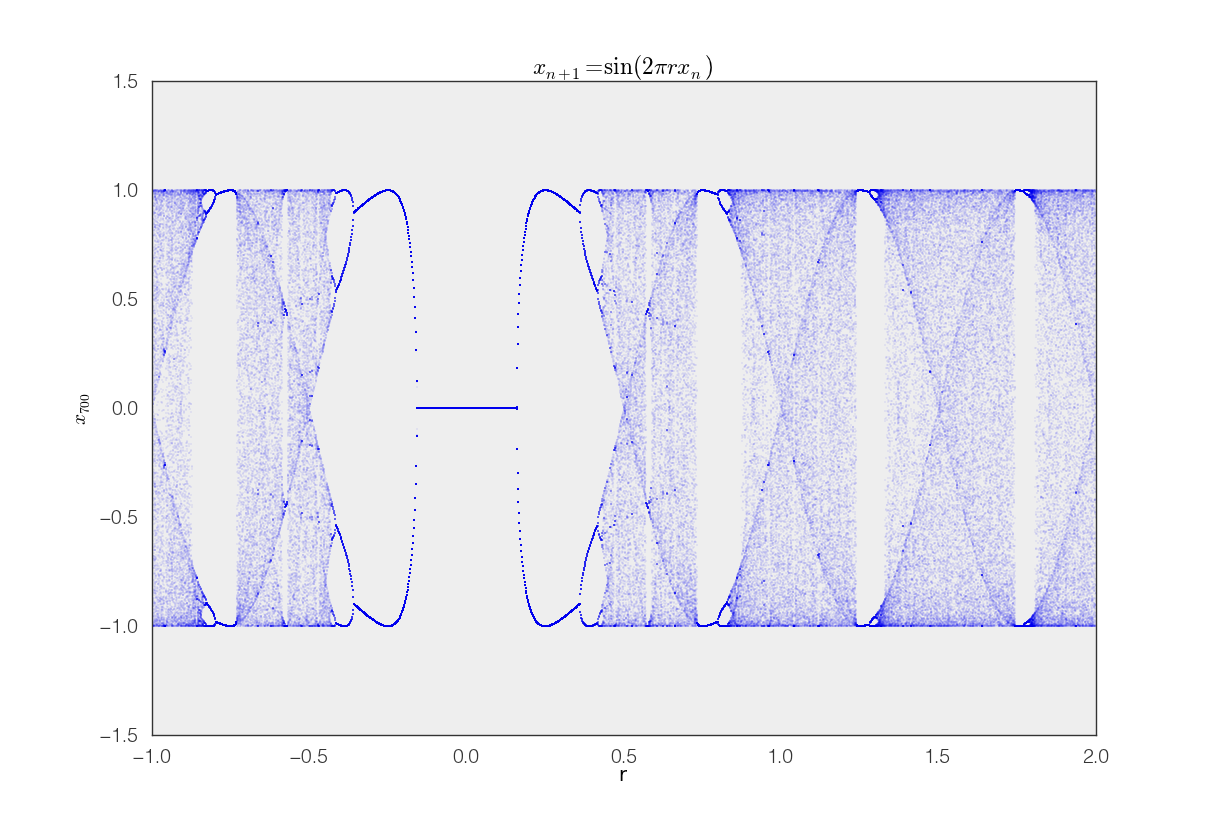
\includegraphics[width=\textwidth]{sin}
  \caption{Bifurcation diagram for the trigonometric map: $x_n \rightarrow \sin (2 \pi x_n)$}
  \label{fig:trig}
\end{figure}

\pagebreak

\section{Strange Attractors}
\label{sec:strng}

We can see in the bifurcation diagram of the logistic
map(Fig.~\ref{fig:logmap}) that even in the ``chaotic'' regions, there
appears to be some lines through the mess that trace out what might
seem to be more probable points. There exists an exact solution to the
logistic map(Eq.\ref{eq:logmap}) for $r=4$, so we can more closely
examine this map at this value. 

\vline

We begin by making the substitution
\begin{equation}
  \label{eq:sub}
  x_n \rightarrow \sin^2(\pi \theta_n) = \frac{1}{2}[1-\cos(2\pi \theta_n)]  
\end{equation}
This gives that $\theta_{n+1} = 2\theta_n$ and consequently $\theta_n
= 2^n\theta$. We can also see that $x$ is also periodic in $\theta$,
in that integer shifts in $\theta$ yield the same $x$. We can now
consider a seed value of $\theta_0$ to be generated by the sum of the
inverse powers of 2 ($\theta_0 =
\frac{1}{2}+\frac{1}{8}+\frac{1}{16}+\frac{1}{64}+...$). Because we
can truncate the integer part of the decimal representation of the
$\theta_n$'s due to the periodicity of the $x_n$'s, we see that each
digit of the $\theta_n$'s is either a 0 or a 1 with equal probability,
and so we find that the $\theta$ is uniformly distributed across its
seed values on $[0,1]$. Since $\theta$ is distributed uniformly, $x$
must obey some non-uniform distribution because of how $x$ is defined
in terms of $\theta$. We get that the $x$'s obey the distribution
\begin{equation}
  \label{eq:dist}
  P(x) = \frac{1}{\pi\sqrt{x(1-x)}}
\end{equation}
This would suggest that $x$ is more concentrated around 0 and 1, which
we see is the case in Figure~\ref{fig:logmap}. Instead of the
attractor being a point or cycle of points, the distribution, $P(x)$
is the attractor. These distribution attractors exist for other values
of $r$ and can also be seen roughly in Figure~\ref{fig:logmap} and
\ref{fig:trig}, and are referred to as \emph{strange attractors}.

\subsection{The Lorenz Attractor}
\label{sec:lor}

Edward Lorenz\cite{lorenz} was interested in modeling the macroscopic
flow of the Earth's atmosphere as a function of time. He developed a
system of differential equations, the \emph{Lorenz System}, from the
\emph{Navier Stokes Equations} to model this system. The coupled
equations are as follows:
\begin{align}
  \label{eq:lorenz}
  \begin{split}
    \frac{dx}{dt} &= \sigma (y - x) \\
    \frac{dy}{dt} &= x(\rho - z) - y \\
    \frac{dz}{dt} &= xy - \beta z
  \end{split}
\end{align}
The story goes that Lorenz had allowed his computer to truncate the
results to a few digits to save time printing results, and a
difference of only 10$^{-3}$ he found wildly diverging
results. Figures~\ref{fig:lorenzc} and \ref{fig:lorenzd} show how a
difference in initial conditions of 10$^{-4}$ can create a very
divergent time evolution. Figure~\ref{fig:lorenz} also shows how
regardless of the initial conditions the curve, over time, is
attracted to the same two circular curves, even though it sweeps them
out in irregular ways, differing in time.


\begin{figure}
        \centering
        \begin{subfigure}[b]{0.5\textwidth}
                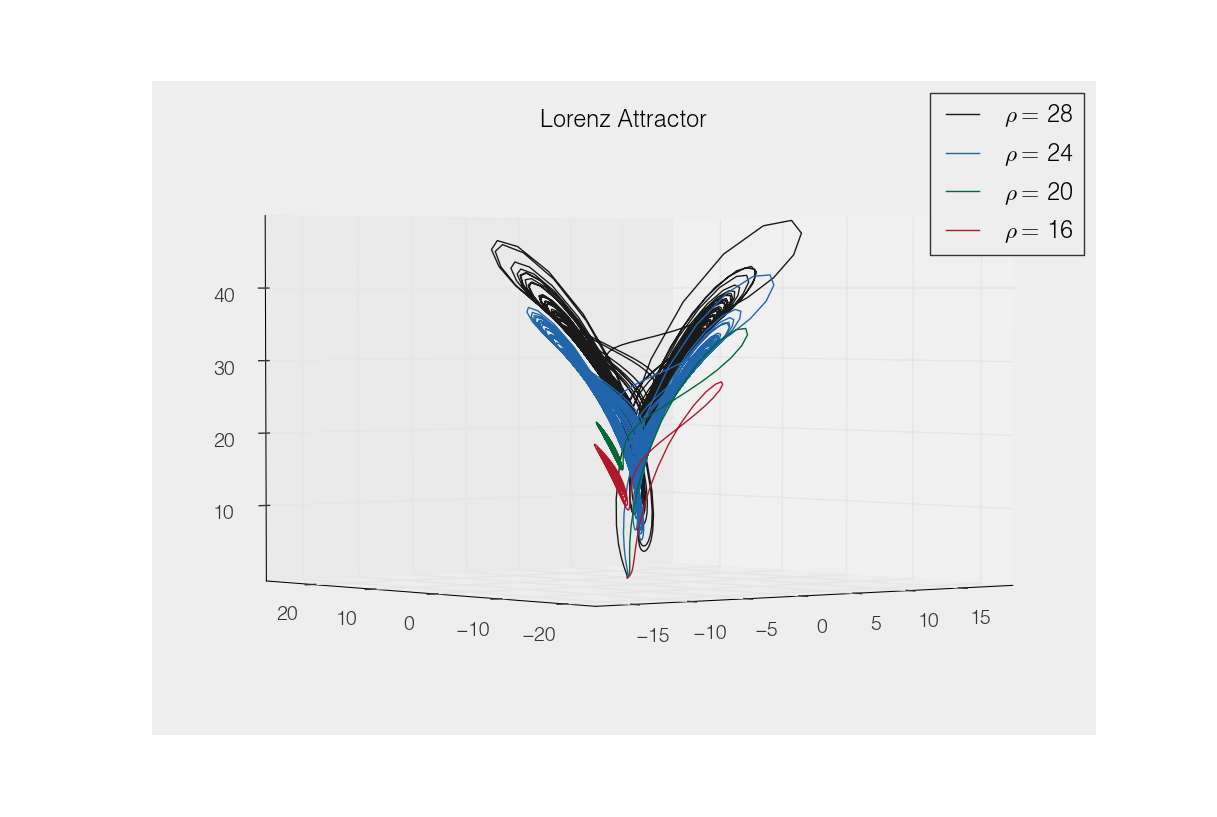
\includegraphics[width=\textwidth]{lorenz1}
                \caption{Various initial conditions}
                \label{fig:lorenza}
        \end{subfigure}%
        ~ %add desired spacing between images, e. g. ~, \quad, \qquad etc.
          %(or a blank line to force the subfigure onto a new line)
        \begin{subfigure}[b]{0.5\textwidth}
                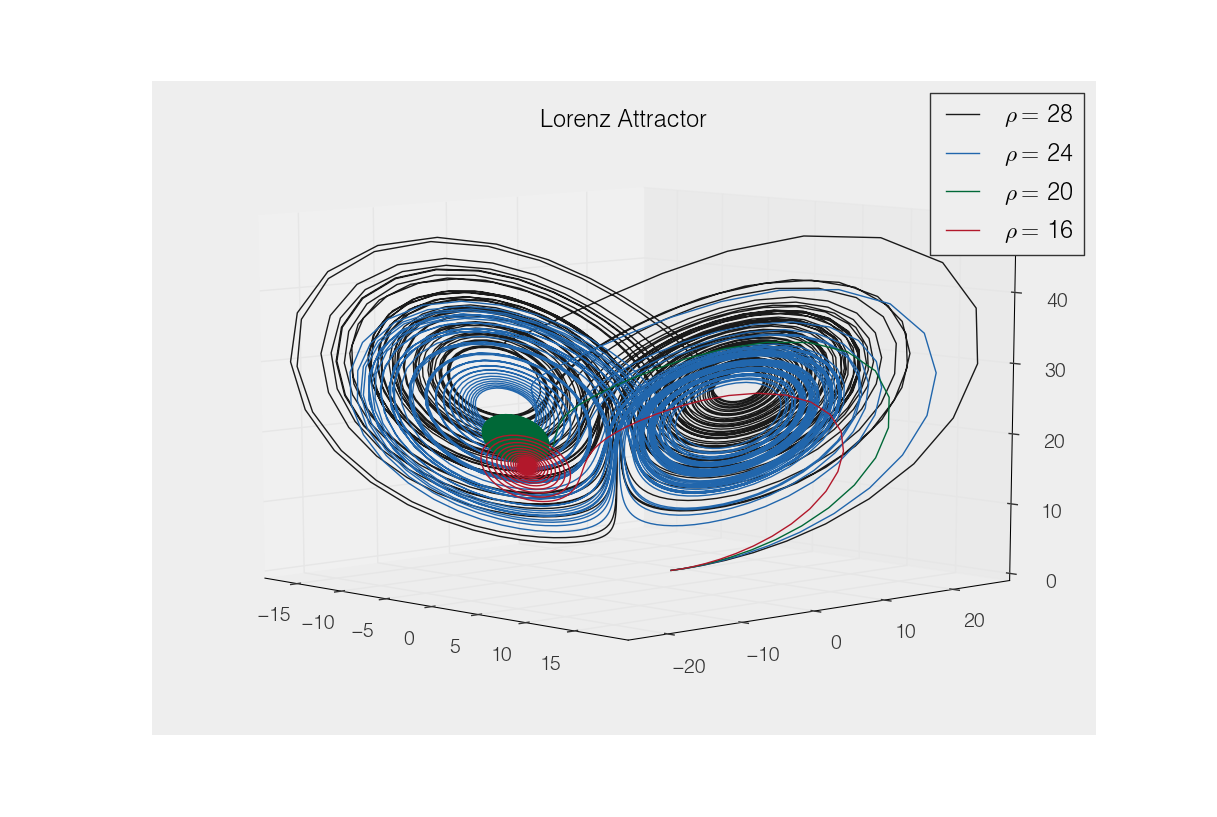
\includegraphics[width=\textwidth]{lorenz_z0}
                \caption{Various initial conditions}
                \label{fig:lorenzb}
        \end{subfigure}
        ~ %add desired spacing between images, e. g. ~, \quad, \qquad etc.
          %(or a blank line to force the subfigure onto a new line)
        \begin{subfigure}[b]{0.45\textwidth}
                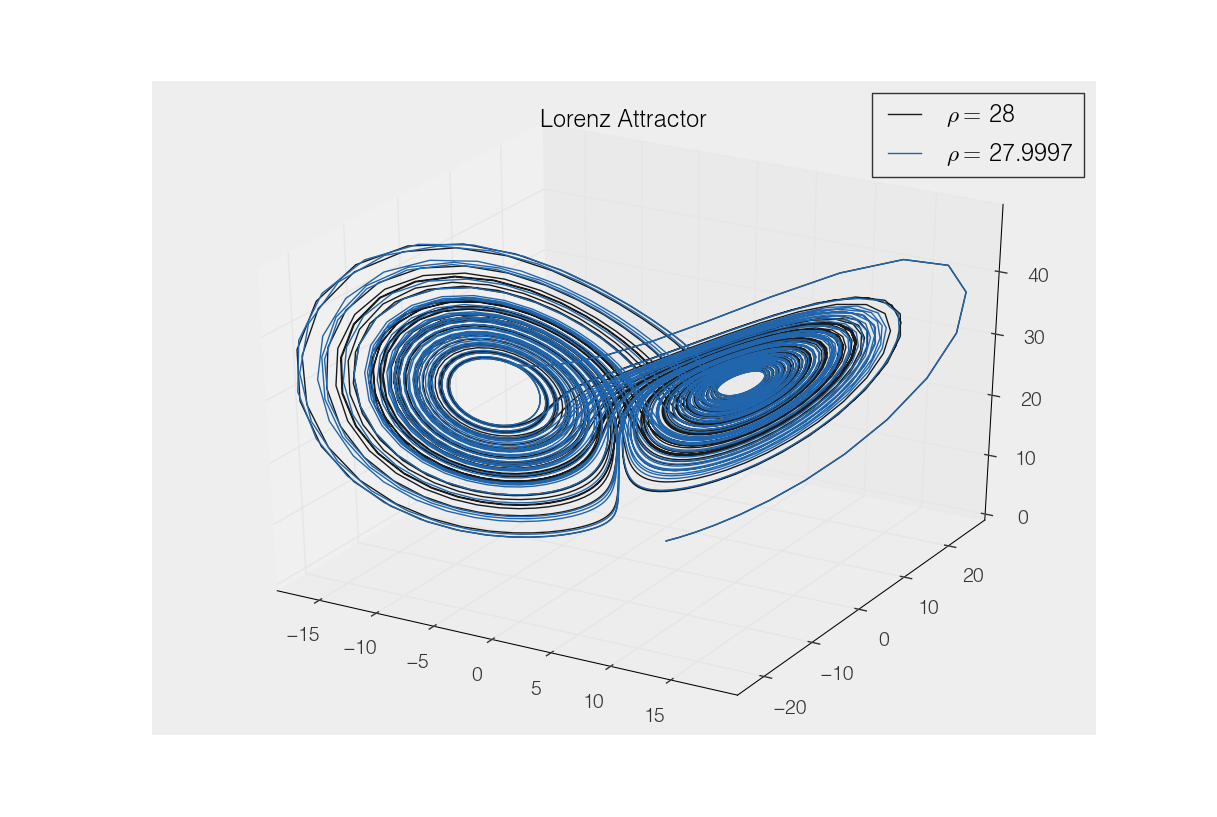
\includegraphics[width=\textwidth]{lorenzsmallosc}
                \caption{Small Fluctuations in initial conditions}
                \label{fig:lorenzc}
        \end{subfigure}
        \begin{subfigure}[b]{0.45\textwidth}
                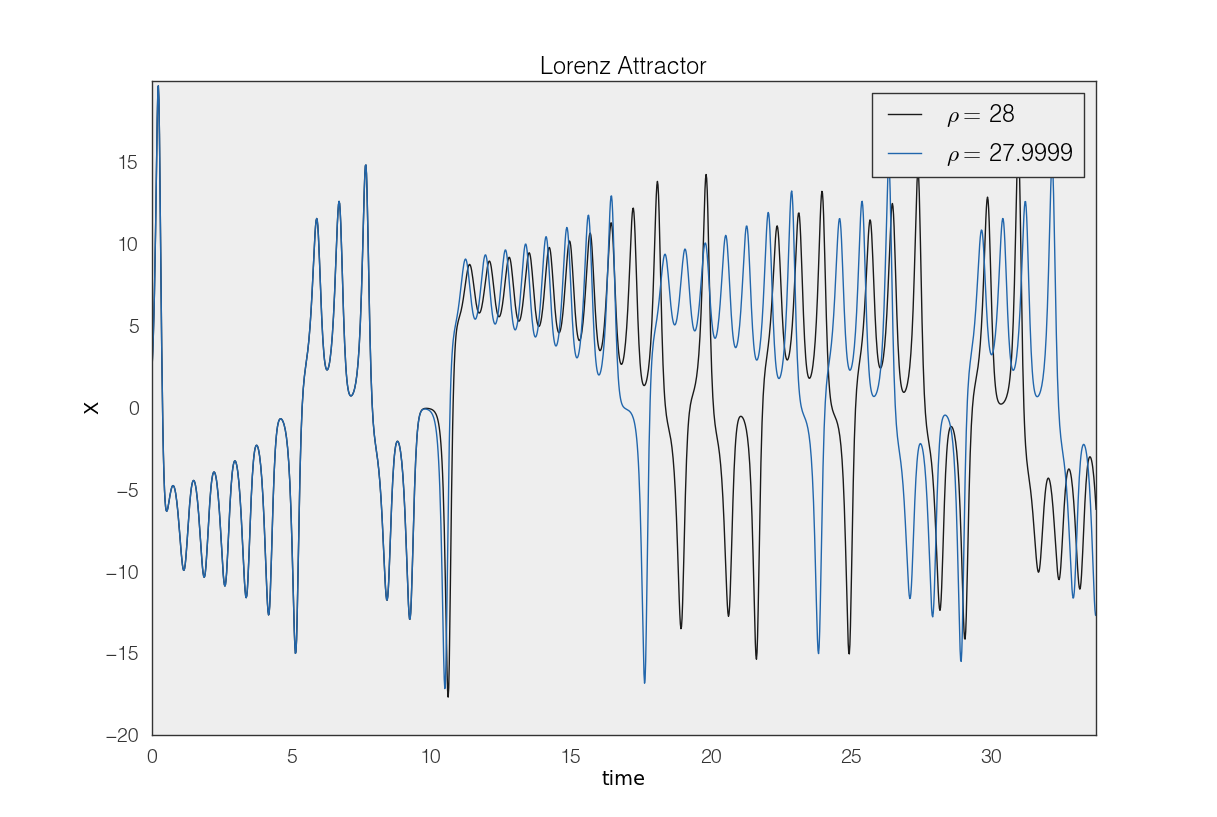
\includegraphics[width=\textwidth]{lorenzx}
                \caption{X from Figure~\ref{fig:lorenzc} plotted
                  against time}
                \label{fig:lorenzd}
        \end{subfigure}

        \caption{Time Evolution of the Lorenz System for initial
          conditions $x=2,y=5,z=0,\sigma =10, \beta = 8/3$}\label{fig:lorenz}
\end{figure}

\subsection{The R\"{o}ssler Attractor}
\label{sec:ross}

Otto R\"{o}ssler created a system of non-linear differential equations
intended to behave like the Lorenz Attractor, but be easier to
analyze\cite{rossler}. The system has been since found to model the
equilibrium of some chemical reactions. The equations are as follows:
\begin{align}
  \label{eq:rossler}
  \frac{dx}{dt} &= -y - z\\
  \frac{dy}{dt} &= x + ay \\
  \frac{dz}{dt} &= b + z(x-c)
\end{align}

\begin{figure}
        \centering
        \begin{subfigure}[b]{0.7\textwidth}
                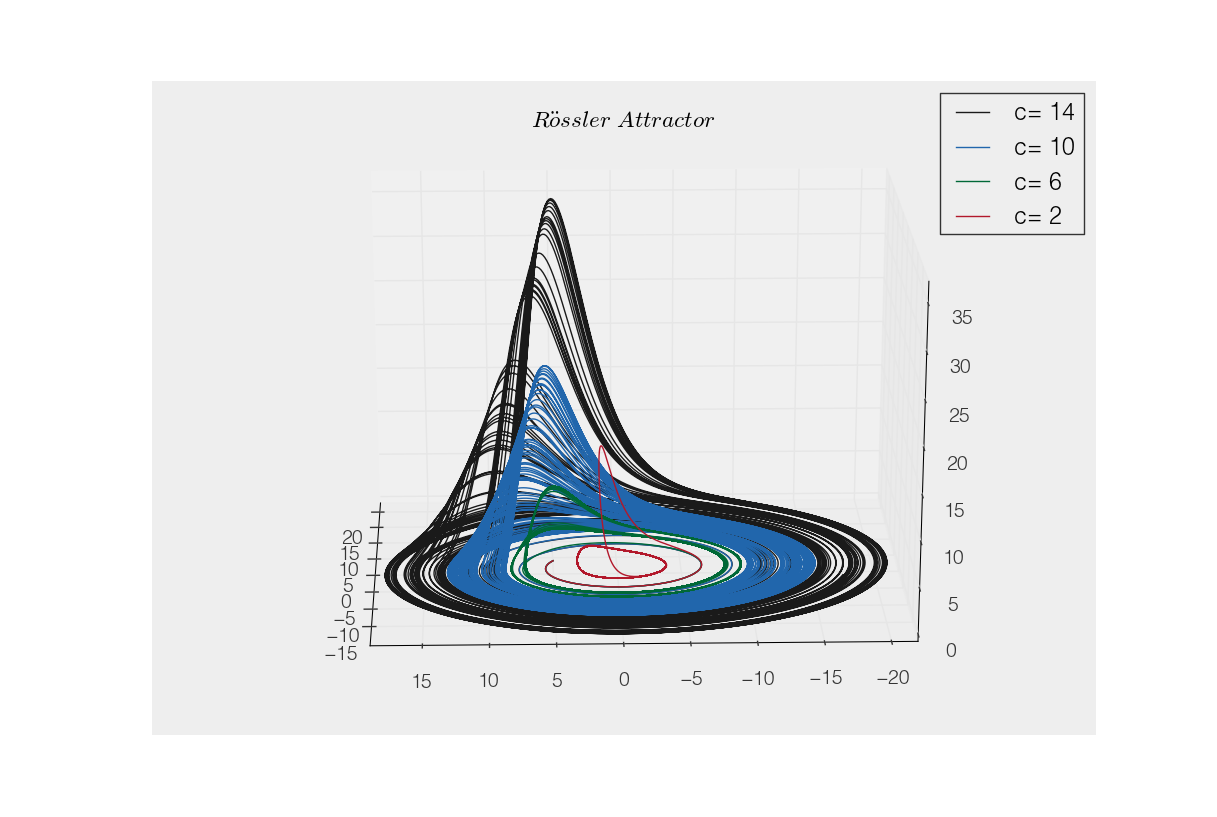
\includegraphics[width=\textwidth]{rossler}
                \caption{Various initial conditions}
                \label{fig:rosslera}
        \end{subfigure}%
        \hspace{1mm}
        \begin{subfigure}[b]{0.7\textwidth}
                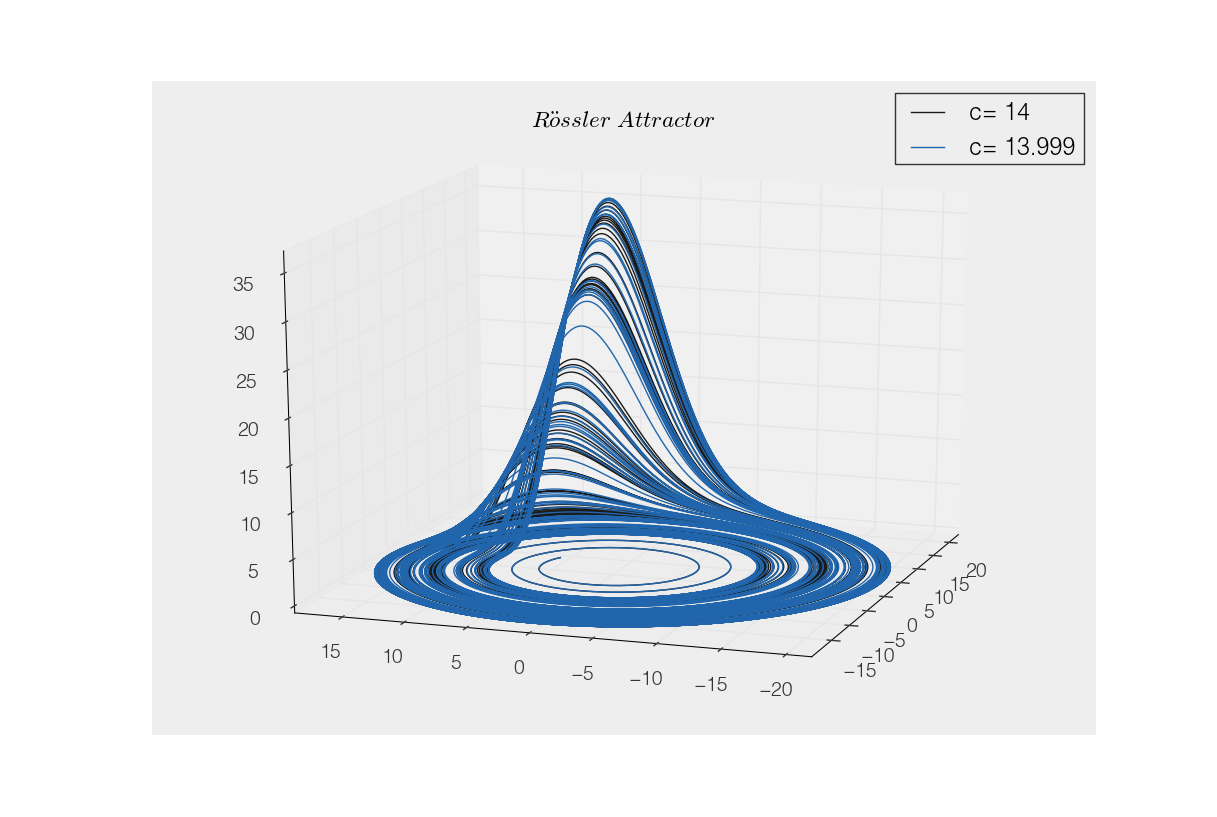
\includegraphics[width=\textwidth]{rossler2_3d}
                \caption{Small Fluctuations in initial condidtions}
                \label{fig:rosslerb}
        \end{subfigure}
        ~ %add desired spacing between images, e. g. ~, \quad, \qquad etc.
          %(or a blank line to force the subfigure onto a new line)
        \begin{subfigure}[b]{0.7\textwidth}
                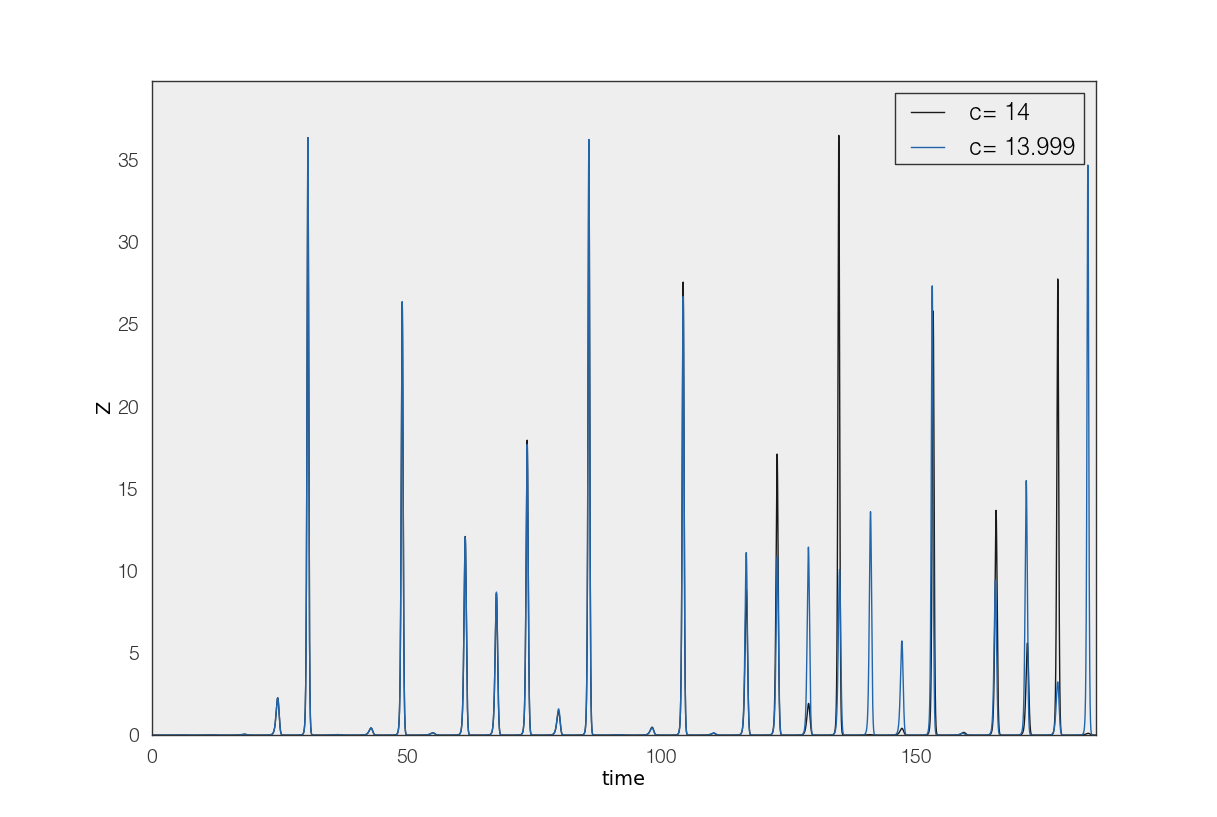
\includegraphics[width=\textwidth]{rossler2}
                \caption{Small Fluctuations in initial conditions. }
                \label{fig:rosslerc}
        \end{subfigure}
        \caption{Time Evolution of the R\"{o}ssler System for initial
          conditions $x=2,y=5,z=0,a =0.1, b = 0.1$}\label{fig:rossler}
\end{figure}

We see in Figure~\ref{fig:rossler} that again our system is extremely
sensitive to initial conditions. Our system is drawn to circles in the
$xy$ plane and some periodic spirals in the $z$ direction. We see in
Figure~\ref{fig:rosslerc} that the timing of these $z$ fluctuations
varies greatly even with small fluctuations in initial conditions.

\newpage

\appendix

\section{Source Code}
\label{sec:src}



All programs used to generate the plots shown in this paper are available online at
\url{https://github.com/acreyes/Dynamics}. The repository contains the
following programs:
\begin{itemize}
\item bi.py - Creates the bifurcation diagram plots
\item rossler.py - Plots the R\"{o}ssler attractor for various initial
  conditions
\item lorenz.py - Plots the Lorenz attractor for various initial conditions
\end{itemize}

The plots for the Lorenz and R\"{o}ssler attractors were made by using
a fourth order Runge-Kutta numerical method(as found in\cite{numerical}) to solve the
Lorenz and R\"{o}ssler equations. 





%\lstinputlisting[label=bi,caption=Program to make bifurcation
%plots, width = .9\textwidth]{bi.py}

%\lstinputlisting[label=rossler,caption=Program to plot Rossler Attractor, width = .9\textwidth]{rossler.py}

%\lstinputlisting[label=lorenz,caption=Program to plot Lorenz Attractor, width = .9\textwidth]{lorenz.py}


\bibliographystyle{plain}
\bibliography{references}

\end{document}